\section{PCA}

\textbf{PCA} uses an orthogonal transformation (vectors multiplied are 0) to
convert a dataset with maybe correlated datas into a dataset without
correlations.

The first component has to satisfy the following:

\begin{align*}
w_1 &= \text{argmax}_{||w|| = 1} \{\sum_i (t_1)_i^2\}\\
	&= \text{argmax}_{||w|| = 1} \{\sum_i (x_iw)^2\}\\
\end{align*}
Which is achieved by the corresponding eigenvector.

The next components need to fullfill:
\begin{align*}
\hat{X}_k &= X - \sum_{s=1}^{k-1} Xw_sw_s^T\\
w_k &= \text{argmax}_{||w|| = 1} \{||\hat{X}_kw||^2\}\\
	&= \text{argmax}_{||w|| = 1} \{\frac{w^T\hat{X}_k^T\hat{X}_kw}{w^Tw}\}\\
\end{align*}

Based on the "weight matrix" a mapping is possible from the original space to a new space in which the dataset is uncorrelated. Also the dimension can be reduced on this manner.


Rapidminer has a tool applying the PCA algorithm on a given dataset. The Output are 
new attributes, which are a combination of the old ones. 

\subsection{Rapidminer Process}
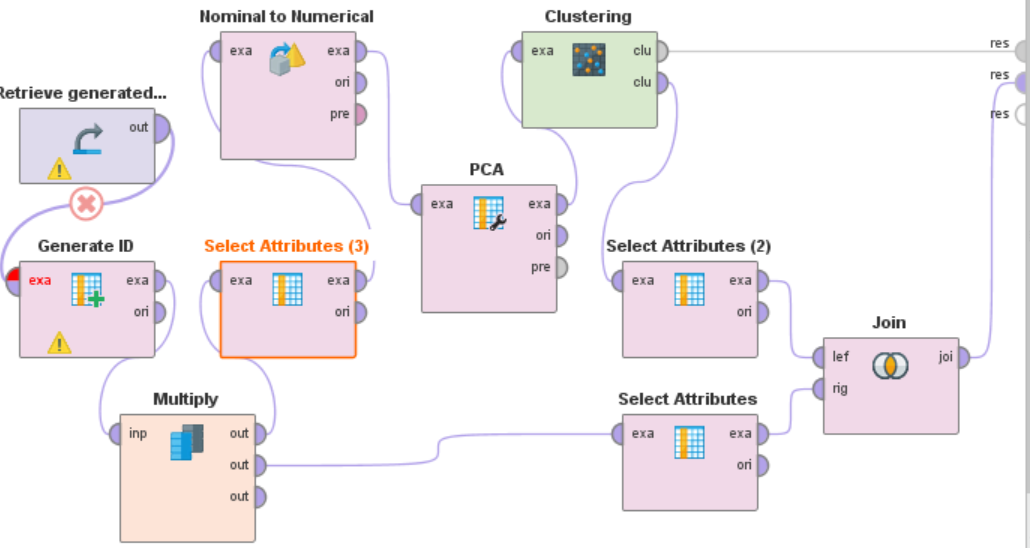
\includegraphics[width=0.9\textwidth]{PCAClustering}

The Process does the following steps:
\begin{description}
	\item[Retrieve] This Block gives the data in the process. For the comparison at the end we also retrieve the original data.
	\item[Nominal to Numerical] This changes the nominal data to numerical data, so that we can apply PCA in the next step
	\item[PCA] Here we apply the PCA reduction to the data with a variance threshold $0.95$
	\item[Clustering] Here the number of Clusters has to be fixed. We decided, that 10 runs should be enough. We can choose between differen measure types and tried mixed euclidean and squared euclidean distance
	\item[Select Attribute] Here we just pick the Strata data for comparing with the clustering
	\item[Join] For comparing the Clustering and the Strata we join the two filtered data sets at the ID
\end{description}

This is the basis for all datasets, where we set the role of id to id by adding the dataset to RapidMiner.

\subsection{Searching for 6 Clusters}

The first idea is to check, if on this way a clustering can be found, comparable to the strata groups. So we use the process for different datasets.

\subsubsection{Applying on original data}
Applying the PCA module on the original data without strata and a variance
threshold of 0.95 we get two Attributes, so we can assume, that the data is strongly connected. As expected the computating time decreases a lot. 

For a clustering of 6 clusters we get a distributions that are complete different.\ref{fig:OrgDist}
\begin{figure}[h]
\centering
\begin{subfigure}{.5\textwidth}
  \centering
  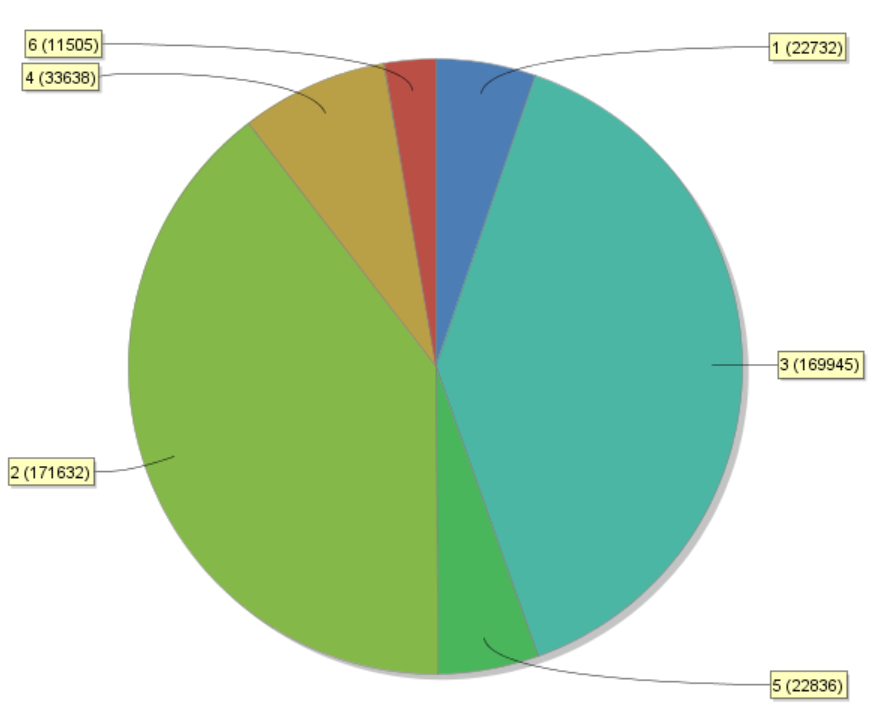
\includegraphics[width=.4\linewidth]{ClusterOrigRapidStrata.PNG}
  \caption{Strata}
  \label{fig:OrgSt}
\end{subfigure}%
\begin{subfigure}{.5\textwidth}
  \centering
  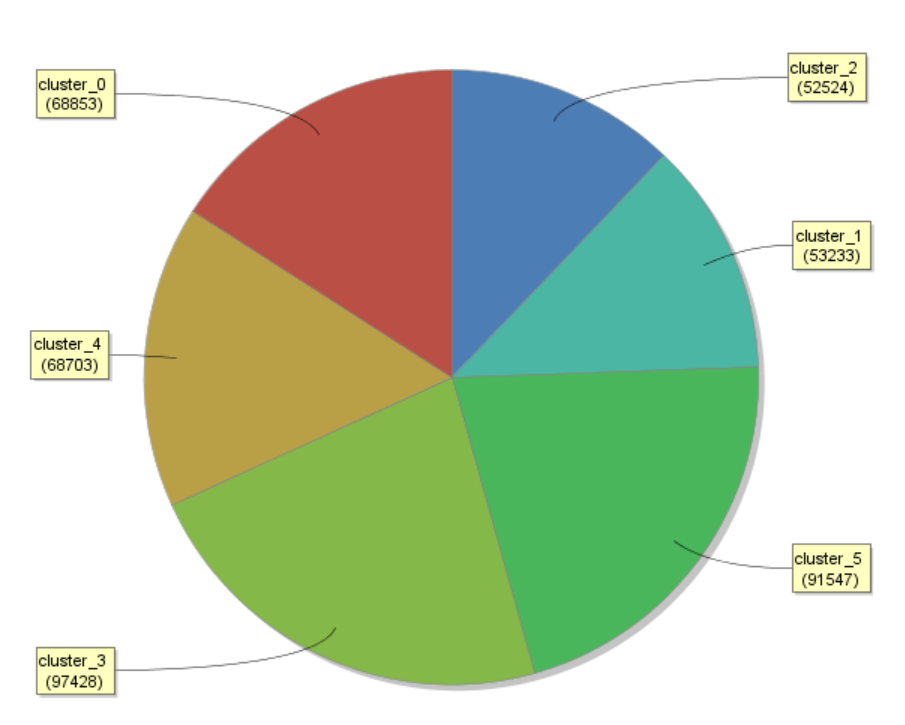
\includegraphics[width=.4\linewidth]{ClusterOrigRapidCluster.PNG}
  \caption{Cluster}
  \label{fig:OrgCl}
\end{subfigure}
\caption{Distribution of original data}
\label{fig:OrgDist}
\end{figure}

Also the distribution in the strata groups of the clustering shows, that there is no real connection of strata and the clustering.
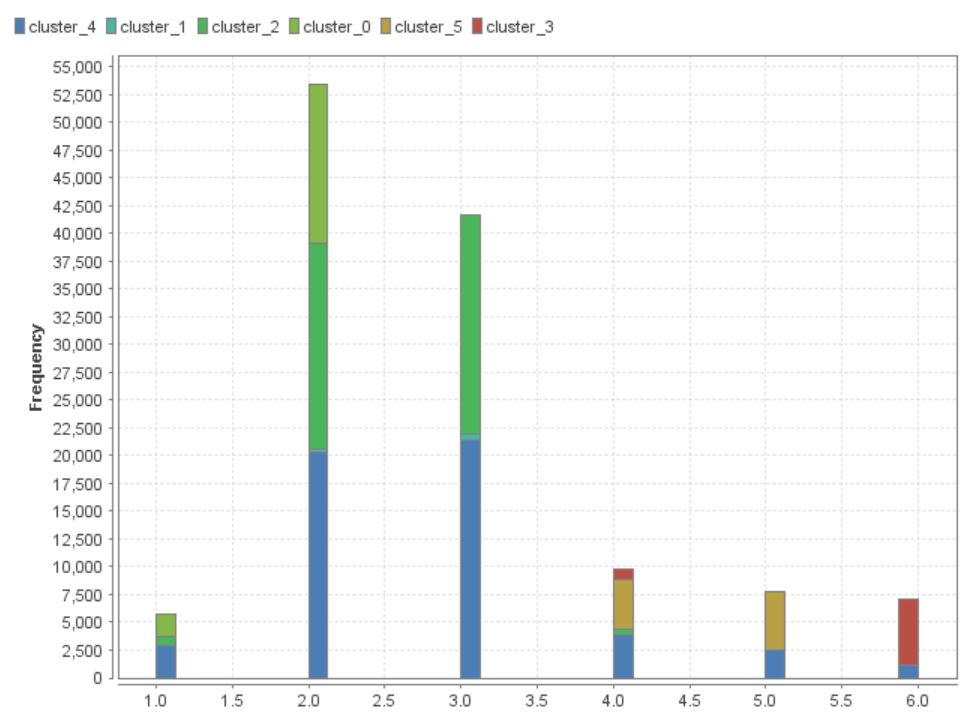
\includegraphics[width=0.9\textwidth]{ClusterPCAOrigRapidDistribution.PNG}

\subsection{Searching for 3 Cluster}

The next idea is, that there are maybe just 3 obvious cluster to see and contain two 2 strata.

\subsubsection{Applying on original data}
Applying the PCA module on the original data without strata and a variance
threshold of 0.95 we get two Attributes, so we can assume, that the data is strongly connected. As expected the computating time decreases a lot. 

For a clustering of 6 clusters we get a distributions that are complete different.\ref{fig:OrgDist}
\begin{figure}[h]
\centering
\begin{subfigure}{.5\textwidth}
  \centering
  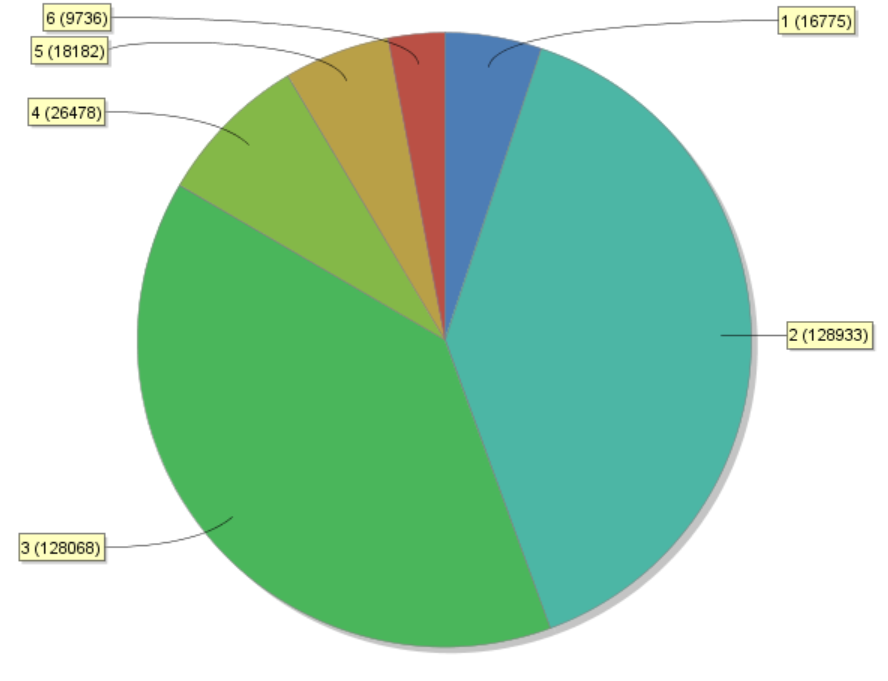
\includegraphics[width=.4\linewidth]{ClusterPCAOrigRapidStrata2Cluster.PNG}
  \caption{Strata}
  \label{fig:OrgSt}
\end{subfigure}%
\begin{subfigure}{.5\textwidth}
  \centering
  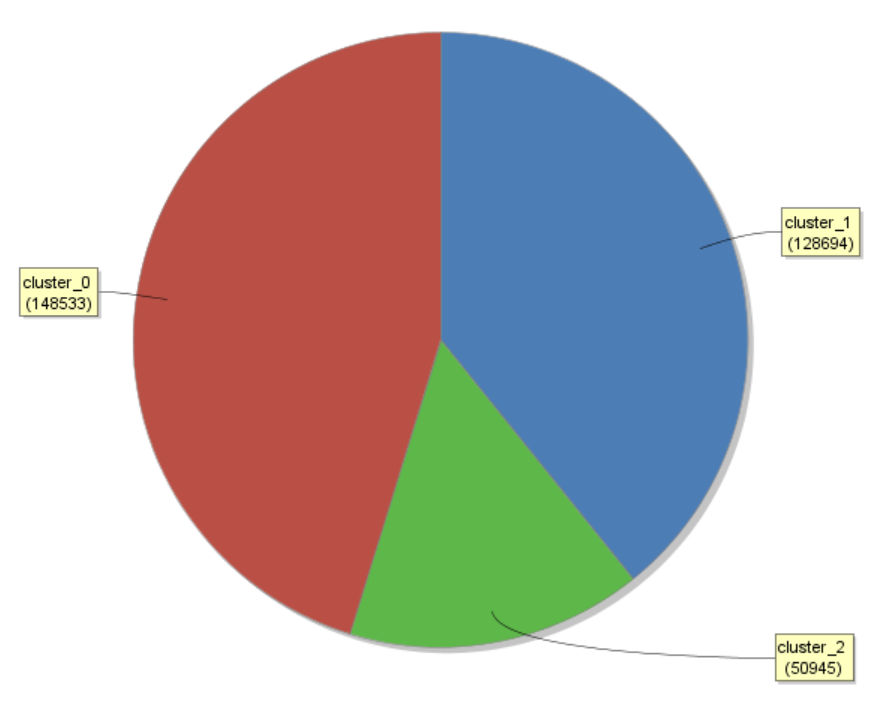
\includegraphics[width=.4\linewidth]{ClusterPCAOrigRapidCluster2Cluster.PNG}
  \caption{Cluster}
  \label{fig:OrgCl}
\end{subfigure}
\caption{Distribution of original data}
\label{fig:OrgDist}
\end{figure}

Also the distribution in the strata groups of the clustering shows, that there is no real connection of strata and the clustering.
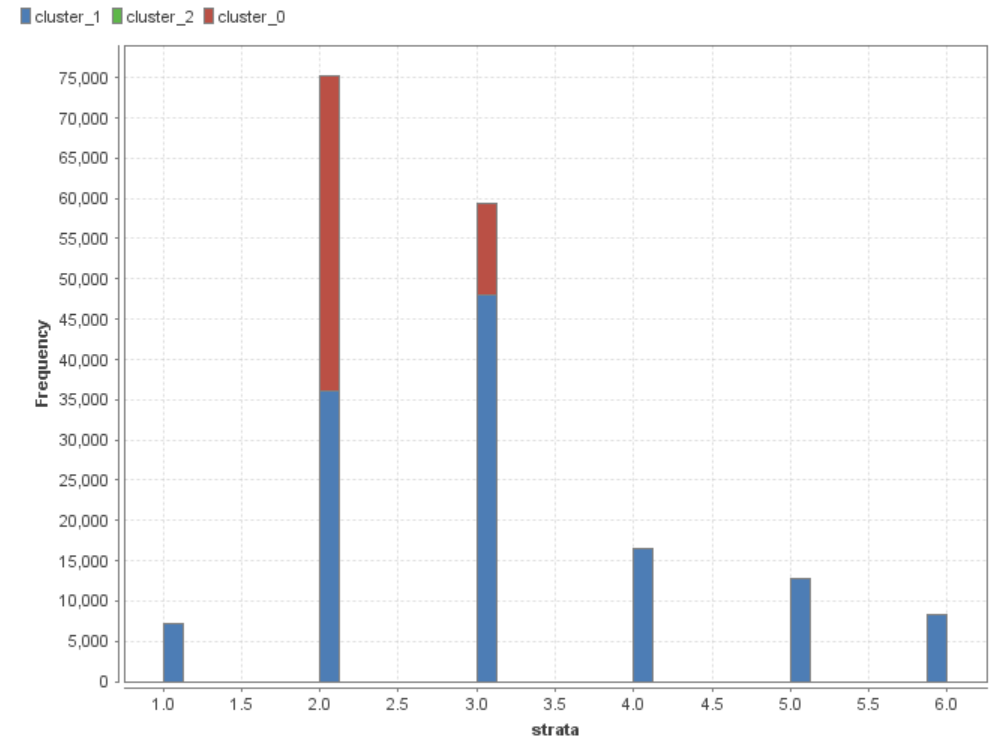
\includegraphics[width=0.9\textwidth]{ClusterPCAOrigRapidDistribution2Cluster.PNG}
